%\chapter{Analysis and Design}
\chapter{Analiză și proiectare}
\label{cap:analiza-si-proiectare}

În acest capitol este descris design-ul proiectului și cuprinde: cerințele sistemului, specificațiile cazurilor de utilizare, arhitectura sistemului, comportamentul sistemului, datele utilizate de sistem, dependințele sistemului și algoritmii esențiali și metodele folosite. Descrierea acestora se realizează prin asocierea cu diagramelor aferente. 

\section{Cerintele sistemului}

Sistemul propus \textit{\thesistitle}  reprezintă un software gratis care oferă clientului atât caracteristici specificie unui reverse proxy, cât și modalități de protecție asemeni unui sistem de prevenire a intruziunilor. 
Sistemul este ușor de instalat și de utilizat, chiar și de către utilizatorii neexperimentați, oferindu-le acestora o interfață clară și sugestivă, ce maschează logica complicată din spate. În spate, sistemul oferă un reverse proxy ce interceptează tot traficul destinat către un anumit server, de pe una sau mai multe interfețe. În procesul de interceptare, acesta implementează și câteva modalități de prevenire a unor tentative de intruziune. Sistemul blochează toți clienții ce folosesc adrese IP aflate pe o lista neagră (IP-urile utilizate frecevent de rețeaua Tor) și reqest-uri ce prezintă un URI cu conținut malițios (atacurile de SQL injection). 

Sistemul trebui să îndeplinească următoarele cerințe  \textbf{functionale}:
\begin{enumerate}
	\item Să realizere conexiunea la un server HTTP/HTTPS și să redirectioneze traficul primit către acesta. 
	\item Să intercepteze traficul venit pe o anumită interfață și port prestabilit. 
	\item Să prelucreze request-urile primite de la clineti într-un format specific pentru clasificatorul de URI-uri. 
	\item Să nu redirectioneze reqesturile clasificate că și malițioase. 
	\item Să blocheze conectarea clienților ce folosesc IP-uri conținute de lista neagră de referință. 
	\item Să permită utilizatorului să editez și să vizualizeze lista adreselor IP blocate. 
	\item Să prezinte în interfața grafică toate intervențiile rezlizate asupra traficului(blocări de conexiuni sau de request-uri). 
	\item Să permită utilizatorului să configureze modul de operare al sistemului. 
\end{enumerate}

Sistemul trebuie, de asemenea, să aibă următoarele caracteristici \textbf{non-funcționale}:
\begin{enumerate}
	\item Să fie ușor de instalat și de folosit pentru orice utilizator, oricât de neexperimentat. 
	\item Să poată intercepta traficul de pe orice/oricâte interfețe disponibile. 
	\item Să poată rula pe orice sistem de operare Windows cu Python2 instalat. 
	\item Să aibă o rată de blocare de 100\% a IP-urilor de pe lista neagră, iar 
	în cazul detecției de SQL injection să nu aibă detecții false pozitive mai mari 2-3\% 
	și o acuratețe generală de peste 90\% 
\end{enumerate}
\newpage

\section{Specificatiile cazurilor de utilizare}

\subsection{Actori, stakeholders si interese}

Principalii actori și stakeholder-i sunt administratorii de servere, respectiv de baze de date. În implementarea sistemului propus se urmărește satisfacerea nevoilor acestor persoane, oferindu-le un plus de securitate asupra datelor ce sunt accesate de către clienți, respectiv împotriva clienților rău intenționați. Interesele acestor comunități de utilizatori sunt urmărite pentru a livra un produs care să ofere aceste protecții într-o manieră cât de prietenoasă pentru utilizator și cât mai eficientă. 

\subsection{Basic flow}

\begin{figure}[h]
	\centering
	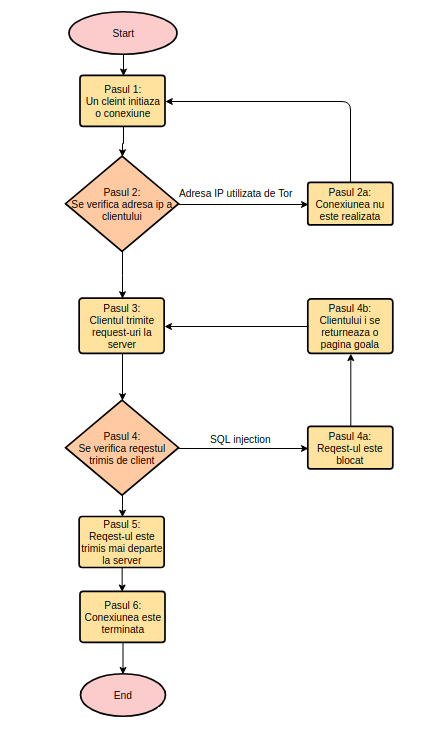
\includegraphics[width=0.4\textwidth]{basicflow.png}
	\caption{Basic flow pentru evenimente}
	\label{fig:basic-flow}
\end{figure}
Figura ~\ref{fig:basic-flow}  prezintă cum arată basic flow-ul pentru evenimentele din sistemul propus. \\
\newpage
Evenimentele sistemului:
\begin{enumerate}
	\item \textbf{Start}: aceste cazuri de utilizare sunt inițiate în momentul în care sistemul este plasat între un server și utilizatorii acestuia. 
	\item \textbf{Pasul 1}: un client dorește și inițializeze o conexiune la server. 
	\item \textbf{Pasul 2}: adresa IP a clientului este verificată că acesta să nu fie un utilizator de Tor. 
	\item \textbf{Pasul 3}: clientul comunică cu serverul prin reqest-uri individuale. 
	\item \textbf{Pasul 4}: reqest-urile sunt verificate că acestea să nu fie atacuri de SQL injection. 
	\item \textbf{Pasul 5}: request-urile sunt trimise mai departe către server. 
	\item \textbf{Pasul 6}: conexiunea este terminată(de către client sau server). 
	\item \textbf{End}: la sfârșitul unui șir de evenimente, utilizatorul sistemului poate să vadă dacă clientul ce a inițializat evenimentele a realizat acțiuni considerate ca malițioase. 
	
	
\end{enumerate}


\subsection{Alternative flow}
Evenimentele alternative în cazurile de utilizare sunt următoarele: 
\begin{enumerate}
	\item \textbf{Pasul 2a}: în cazul în care un utilizator cu adresă IP de Tor încearcă să realizeze conexiunea la server aceasta este refuzată.  
	\item \textbf{Pasul 4a}: în cazul în care un utilizator încearcă să trimită la server un request ce reprezintă o tentativă de atac SQL injection, acesta este blocat. 
	\item \textbf{Pasul 4b}: pentru request-urile blocate ca și SQL injection clientului i se returnează o pagină goală. 
\end{enumerate}

\newpage


\section{Arhitectura sistemului si modulele principale}

În conformitate cu cerințele sistemului și specificațiile cazurilor de utilizare, sistemul propus este alcătuit din module specifice care să trateze în mod individual problemele majore ridicate de sistem, printr-o implementare modulară, oferind astfel ușurința implementării de noi funcționalități. 

\begin{figure}[h]
	\centering
	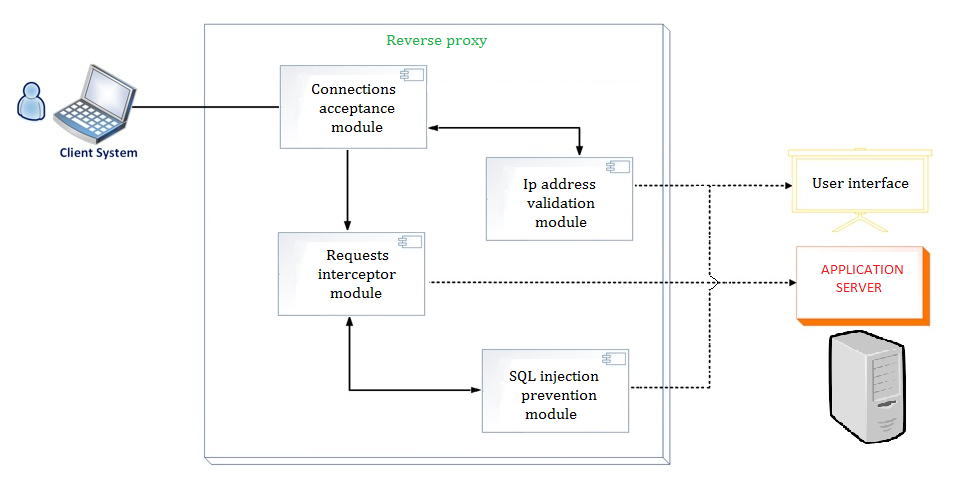
\includegraphics[width=0.8\textwidth]{module.png}
	\caption{Principalele module ale sitemului propus}
	\label{fig:module}
\end{figure}
Figura ~\ref{fig:module}  prezintă care sunt pricipalele module ale sistemului propus, precum și interacțiunea dintre acestea. \\

Principala și teoretic singura componentă a sistemului este reprezentată de cea de \textbf{reverse proxy}, insă pentru a obține rezultatele dorite și pentru a incorpora functionalitătile de protecti în aceasta, logică ei a fost impărtită în cele 4 mari submodule :\textbf{modulul de inițiat conexiuni} și \textbf{modulul de interceptat request-uri}, ce reprezintă componentele ce suportă logica unui reverse proxy și \textbf{modulul de validare a adreselor IP} și \textbf{modulul de validare a URI-urilor}, ce reprezintă modulele care interacționează cu cele ce implementează structura de reverse proxy pentru a oferi funcționalitățile de securitate. \\




\textbf{Sistemul Client} și  \textbf{application server}.\\ 

Aceste două componente reprezintă componetele clasice între care vin plasat sistemul propus. \textbf{Sistemul client} este reprezentat de orice client dorește să acceseze baza de date/partea de server a unei aplicații. \textbf{Application server} reprezintă serverul aplicație la care se pot conecta clienții pentru a avea acces la un anumit conținut. Sistemul propus are rolul de intermediere între cele două tipuri de componente, prevenind astfel eventuale tentative de expluatare a unor vulnerabilități din partea clientului către server.


\textbf{Modulul de inițiat conexiuni}.\\

Acest modul este constituit din componentele oferite de biblioteca open source \textbf{twisted}, fiind modificate ulterior pentru a permite integrarea modulului \textbf{Modulul de validare a adreselor IP} . Modulul are rolul de a crea un socket pe sistemul pe care rulează acesta, care să asculte pentru posibile conexiunui. În cazul în care un client încearcă să inițieze o nouă conexiune acesta trasmite adresa IP a clietului către modulul \textbf{Modulul de validare a adreselor IP}, iar în funcție de răspunsul acestuia conexiunea acestuia va fi realizată sau refuzată. \\ 


 \textbf{Modulul de interceptat request-uri}.\\
 
Asemeni modulului anterior, \textbf{Modulul de inițiat conexiuni}, acest modul este construit peste codul oferit de biblioteca open source \textbf{twisted}. Biblioteca oferă suport pentru interceptarea reqest-urilor dintre un client și server, implementându-se o logică suplimentarea ce încorporează modulul de detecție a atacurilor SQLI( \textbf{Modulul de validare a URI-urilor}). În acest modul se interpretează natura URL-urilor trimise de către client către server.
Interpretarea constând în analiza URI-ului unui request de către modulul de validare a request-urilor, iar în funcție de rezultatul acestuia returnând răspunsuri corespunzătoare atât clientului cât și serverului(în caz de tentatica de atac, la server nu va ajunge nimic).  \\
 
	\textbf{Modulul de validare a adreselor IP}. \\

Rolul acestui modul este de  a valida o adresă IP în conformitate cu adresele conținute pe lista neagră de referință a sistemului. La pornirea sistemului modulul încărca în memorie o lista cu toate adresele IP care trebuie să fie blocate. Această lista este construită la pornirea sistemului pe baza unor date salvate local și reactualizate periodic. Pentru validarea unei adrese, în cazul în care această se află în lista cu IP-uri blocate modulul returnează valoarea "false" codului apelant, iar în caz contrar valoarea "true".  \\

 \textbf{Modulul de validare a URI-urilor}. \\
  
Modulul de validare a URI-urilor este constituit din modelul de detectare a atacurilor SQL injection. Logica modelului de detecție a atacurilor SQL injection este împărțită în două componente. În prima parte acesta indentifică trăsăturile specifice unui atac SQL injection într-un URI. Aceste trăsături sunt reprezentate de caractere și cuvinte cheie ce pot fi găsite în acesta. În cazul indentificarii unor astfel de trăsături, URI-ul este pasat mai departe celei de a doua componentă. Aceasta din urmă este reprezentată de un model de support vector machine antrenat anterior, care va decide dacă URI-ul primit se încadrează în cele specifice atacurilor de SQL injection sau nu. Asemeni modulului anterior \textbf{Modulul de validare a adreselor IP}, în funcție de rezultatul obținut acesta va returna "true" sau "false" codului apelant. 

\section{Comportamentul sistemului. Diagrama de stare si de secventa}
\begin{figure}[h]
	\centering
	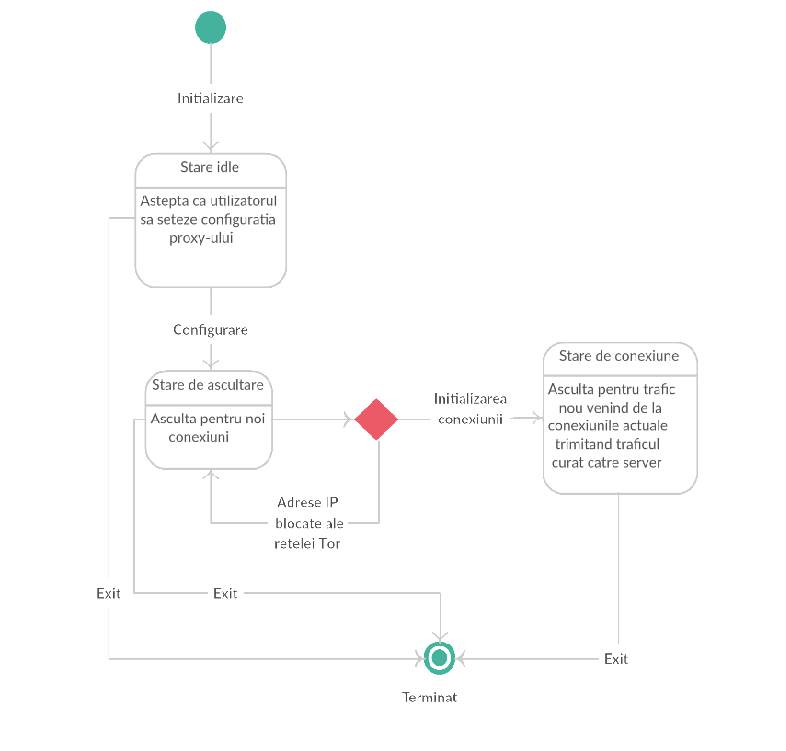
\includegraphics[width=0.8\textwidth]{state_diagram.png}
	\caption{Diagrama de stare a sistemului propus.}
	\label{fig:state}
\end{figure}
Figura ~\ref{fig:state} prezintă diagrama de stare a sistemului propus.

După pornirea aplicației reprezentată prin inițializare, utilizatorului i se pune la dispoziție interfața de utilizator în care sistemul așteaptă să fie configurat și portnit("Stare inactivă"). După configurarea aplicației în meniul "Configure",prin setarea specificațiilor serverului de reverse proxy, prin apăsarea butonului "start", sistemul trece în următoarea stare "Strare de ascultare". În această stare sistemul acceptă noi conexiuni de la diferiți clienți ce doresc să acceseze server-ele protejate de acesta. Tot aici are loc și verificarea adreselor IP ale clienților pentru protejarea importiva utilizatorilor Tor. După stabilirea unei noi conexiuni, sistemul intră în starea "Satre de conexiune", în care acesta ascultă pentru noi request-uri între client și server și le trasmite mai departe către destinația dorită. Tot aici are loc și validarea request-urilor trimise de clienți către server pentru prevenirea atacurilor SQL injection. În această stare utilizatorul poate să urmărească activitatea sistemului în meniul "Monitor" din interfața de utilizator, unde sunt logate toate evenimentele generate de sistem. Pentru oprirea aplicației, utilizatorul poate pur și simplu să o închidă de la butonul din drapta sus, aceasta terminându-și toată activitatea indiferent de starea în care se află. 


\begin{figure}[h]
	\centering
	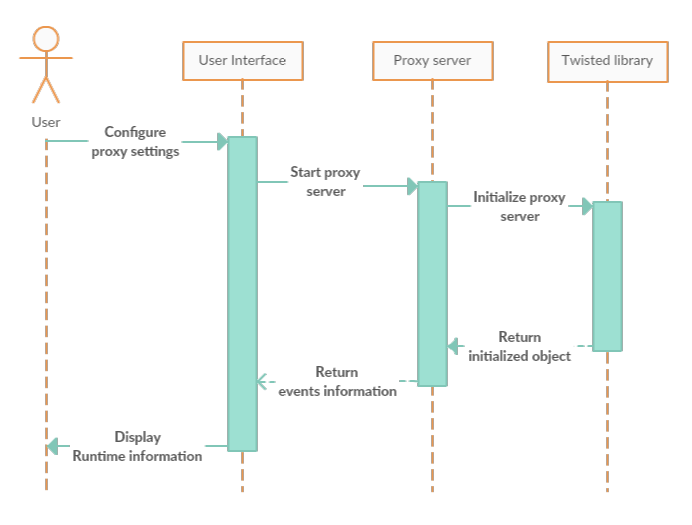
\includegraphics[width=0.9\textwidth]{sequence_diagram.png}
	\caption{ Diagrama de secvența a sitemului propus. }
	\label{fig:sequence}
\end{figure}
Figura ~\ref{fig:sequence}  prezintă diagrama de secvență a sitemului propus.  \\

După pornirea sistemului, utilizatorul configurează setările pentru server-ul de reverse proxy din interfața de utilizator(în meniul "Configure"). După configurarea sistemului, prin apăsarea butonului de start, este lansată în execuție server-ul de reverse proxy cu caracteristicele specificate de utilizator. Scriptul de pornire a server-ului de reverse proxy face apel la fișierele bibliotecii Twisted, care vor returna către acesta o instanță a serverului inițializat. În interiorul server-ului de reverse proxy, apariția de noi evenimente este semnalată către interfața grafică. Aceste evenimente sunt puse la dispoziția utilizatorului pentru vizualizare. 
\\
\section{Dependintele sistemului}

Pentru funcționarea corectă a sistemului propus, acesta are nevoie de următoarele dependințe: 
\begin{enumerate}
	\item Sistem de operare Windows cu Python2 instalat pe sistem. 
	\item Conexiune stabilă la internet pentru rularea script-urilor ce obțin adresele IP utilizate de Tor. 
	\item Sistemul să aibă acces direct la interfețele prin care clienții se pot conecta la server-ul protejat 
	\item Sistemul să aibă o conexiune directă la server-ul ce trebuie protejat. 
\end{enumerate}
\section{Algoritmi si metode}

Pentru prevenirea atacurilor de SQL injection s-a folosit un algoritm de machine learning, support vector machine. Acest algoritm presupune antrenarea anterioară a unui model cu un set de date de referință etichetate în prealabil corect de către utilizator. Aceste date sunt folosite de algoritm pentru a raporta noi seturi de date, natura acestora fiind necunoscută, încercând să găsească similitudin între cele noi și cele de referință, determinându-le astfel natură celor noi. Algoritmul de support vector machine rezultă într-un model obținut prin folosire a diverși algoritmi pentru antrenarea acestuia, folosit pentru a clasifica date. 

Realizarea unui astfel de model sa realizat în urmă executării unui proces elaborat ce implică mai mulți păși: 
\begin{itemize}
	 \item  Primul pas reprezintă indentificarea datelor relevante în cea ce privește problema tratată(prevenirea atacurilor SQL injection). În conformitate cu scopul clasificării evenimentelor/datelor în două categorii (tentativă de atac și request-uri clean) inițial au fost  indentificate o serie de astfel de evenimente și categorizate în evenimente ce sigur aparțin fiecărei dintre categoriile țintă.  
	\item După  obținerea datelor de antrenare, au fost indentificate toate trăsăturile relevante din aceste date, trăsături care să fie cât se poate de specifice fiecărei categorii în parte. Aceste trăsături au reprezentat cuvintele cheie a limbajului SQL dar și caractere specifice folosite frecvent de acesta. 
	\item După obținerea trăsăturilor specifice datelor de antrenare, sa realizat antrenarea modelului folosind un algoritm specific. În cazul proiectului propus s-a folsoit algoritmul gata implementat, furnizat de biblioteca open source LIBSVM \cite{libsvm}. Pentru obținerea modelului datele de antrenare au fost procesate folosind un kernel gausian. Un kernel gausian reprezintă modul în care modelul procesează datele de antrenare astfel încât clasificarea noilor date să fie realizată prin calcularea similarităților dintre acestea și cele de antrenare. În calcularea similarității dintre aceste două tipuri de date, un parametru foare important este sigma. Acest parametru este ales pentru intrg setul de date, iar valoarea lui este diret proporțională cu gradul de similaritate pe care algoritmul îl va asocia la două evenimente/date diferite. 
\end{itemize}

Pentru blocarea IP-urilor utilizate de reteua Tor s-a folosit un script scris în Python3. Programul interoghează periodic(din 6 în 6 ore) informațiile oferite de \textit{Tor Network Status} \cite{tot_status}, salvând uptime-ul fiecărei adrese din ultimele 6 ore. Indentifiacrea adreselor malițioase se face prin însumarea timpului total din ultima lună de uptime, iar cele cu o valoare mai mare de 7 zile sunt considerate malițioase. Blocarea IP-urilor se realizează prin compoararea cu o astfel de lista generată lunar. 

\section{Diagrama de desfasurare}
\begin{figure}[h]
	\centering
	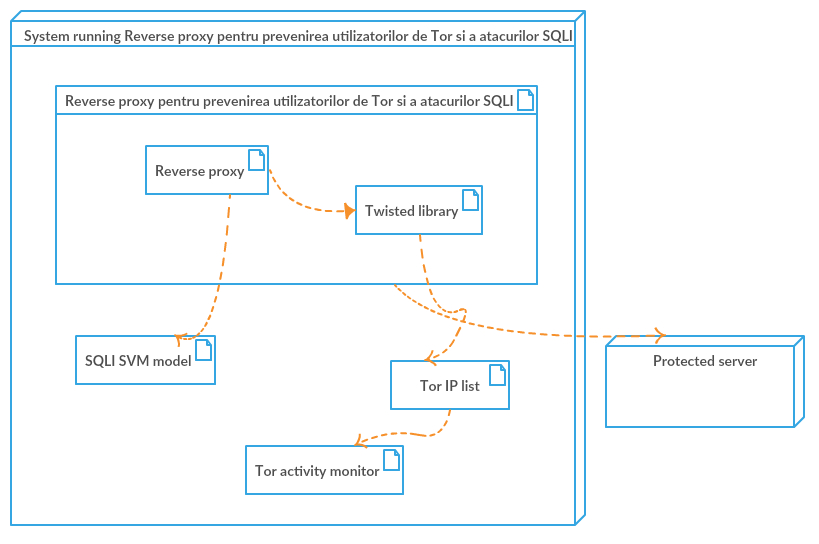
\includegraphics[width=0.8\textwidth]{deployment.png}
	\caption{ Diagrama de desfășurare a sitemului propus. }
	\label{fig:deployment}
\end{figure}

Figura ~\ref{fig:deployment}  prezintă diagrama de desfășurare a sitemului propus.  \\
Pentru a putea rula sistemul \textit{\thesistitle}  pe un sistem, acesta trebuie să aibă acces direct la server-ul ce se dorește a fi protejat. Sistemuli trebuie să îi fie frunizate modelul de SVM folosit pentru prevenirea atacurilor de SQL injection. De asemenea scriptul pentru monitorizarea activității rețelei Tor și cel pentru generarea listei de adrese IP cu un uptime mai mare de 7 zile, trebuie să se afle pe sistem, pentru ca acesta să utilizeze date "up-to-date". 

\section{Justificarea design-ului}
 

 Totate deciziile de design au fost luate în vederea obținerii unor funcționalități cât mai importante pentru utilizatorii țintă, dar și pentru a obține o eficientă cât mai mare a sistemulu, atât din punct de vedere al corectitudinii cât și a timpului de execuție. 


Pentru o acuratețe cât mai mare în prevenirea atacurilor de SQL injection s-a ales folosirea unui abordări bazate pe machine learning, întrucât detecțiile statice prezintă o logică foarte complicată, pot omite multe cazuri esențiale și sunt limitate de capacitatea de observare a programatorului.  


Pentru indentificarea adreselor utilizate de rețeaua Tor se putea aborda o implementare cu lista fixă, întrucât aceste liste prezintă un set mic de adrese ce rămân neschimbate în timp, însă pentru o acuratețe cât mai mare, s-a ales folosirea celor două scripturi suplimentare ce vor obține periodic toate adresele utilizate de rețea în perioada respectivă de timp. 


De asemenea dezvoltarea modulară a sistemului asigură ușurința de adăugare de noi module sau funcționalități fără a necesita modificări majore sistemului actual. 

%Acest capitol descrie design-ul proiectului și cuprinde, în general: 
%\begin{enumerate}
%  \item ilustrarea arhitecturii generale și detaliate a sistemului implementat, care să evidențieze modulele componente și relațiile dintre acestea
%  \item stările prin care trece sistemul în decursul funcționării sale (diagrame de stare)
%  \item modul de interacțiune dintre module și funcționalitatea acestora ilustrată prin diagrame de secvențe
%  \item descrierea algoritmilor/metodelor pe care se bazează funcționarea sistemului dezvoltat
%  \item descrierea organizării/structurii eventualelor baze de date folosite
%  \item justificarea alegerilor/deciziilor făcute și analiza critică a acestora (avantaje și dezavantaje), prin comparație cu alte alternative posibile
%\end{enumerate}
%
%Ca idee generală, design-ul trebuie să fie prezentat independent de o implementare anume, în general, și de cea a voastră, în particular. De asemenea, descrierea design-ului trebuie să conțină toate elementele și detaliile necesare, astfel încât altcineva decât voi să poate realiza o implementare a lui, fără a fi nevoit să ia decizii arhitecturale sau organizare (adică, de design) și să vă contacteze pentru a-și lămuri anumite aspecte neclare.
%
%Capitolul trebuie organizat pe secțiuni și subsecțiuni astfel descrierea să urmeze un cors logic și ușor de urmărit. 
%
%Ponderea acestui capitol relativ la întreaga lucrare este de 25-35\%.
%
%
%\section{Examples: lists, figures, tables, equations}
%
%Așa arată o listă de elemente nenumerotate:
%\begin{itemize}
%  \item element 1
%  \item element 2
%  \item \dots
%\end{itemize}
%
%
%Așa arată o listă de elemente numerotare:
%\begin{itemize}
%  \item element 1
%  \item element 2
%  \item \dots
%\end{itemize}
%
%
%Așa arată o listă în text: 
%\begin{inparaenum}[(\itshape 1 \upshape)]
%  \item element 1, 
%  \item element 2, 
%  \item \dots
%\end{inparaenum}
%
%\textbf{Atenție}: orice tabel, figura sau ecuație (formulă) trebuie referite \textit{explicit} în text explicit (de genul: în Figura X este ulustrat \dots, în Tabelul Y se poate vedea \dots), pentru că Latex le poate plasa chiar și pe altă pagină decât acolo unde vrem noi să ne referim la ele. Vedeți exemple de mai jos!
%
%Tabelul~\ref{table:example} ilustrează un exemplu de tabel. Un editor on-line de tabele poate fi găsit la \url{http://www.tablesgenerator.com/}. 
%
%\begin{table}[t]
%\centering                          % tabel centrat 
%\begin{tabular}{|c|c|c|c|}          % 4 coloane centrate 
%\hline\hline                        % linie orizontala dubla
%Case & Method\#1 & Method\#2 & Method\#3 \\ [0.5ex]   % inserare tabel
%%heading
%\hline                              % linie orizontal simpla
%1 & 50 & 837 & 970 \\               % corpul tabelului 
%2 & 47 & 877 & 230 \\
%3 & 31 & 25 & 415 \\[1ex]           % [1ex] adds vertical space
%\hline                              
%\end{tabular}
%\caption{Nonlinear Model Results}   % titlul tabelului
%\label{table:example}                % \label{table:nonlin} introduce eticheta folosita pentru referirea tabelului in text; referirea in text se va face cu \ref{table:nonlin}
%\end{table}
%
%În Figura~\ref{fig:exemplu} 
%
%\begin{figure}
%    \centering
%    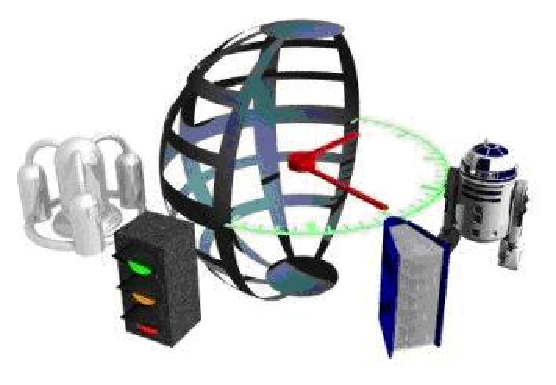
\includegraphics[width=0.5\textwidth]{image}
%    \caption{Numele figurii}
%    \label{fig:exemplu}
%\end{figure}
%
%
%Formula~(\ref{eq:example}) arată modul de calcul al lui $\Delta$:
%\begin{equation} \label{eq:example}
%    \Delta =\sum_{i=1}^N w_i (x_i - \bar{x})^2 .
%\end{equation}
%
%
%Algoritmul~\ref{alg:example} este un exemplu de descriere pseudo-cod a unui algoritm, preluat de la \href{http://en.wikibooks.org/wiki/LaTeX/Algorithms#Typesetting_using_the_algorithm2e_package}{http://en.wikibooks.org/wiki/LaTeX}. El utilizează pachetul \textit{algorithm2e}. Alternativ, puteți utiliza pachetele \textit{algorithmic} sau \textit{program}. 
%
%\begin{algorithm}
% \KwData{this text}
% \KwResult{how to write algorithm with \LaTeX2e }
% initialization\;
% \While{not at end of this document}{
%  read current\;
%  \eIf{understand}{
%   go to next section\;
%   current section becomes this one\;
%   }{
%   go back to the beginning of current section\;
%  }
% }
% \caption{How to write algorithms}
% \label{alg:example}
%\end{algorithm}
